\documentclass[12pt,a4paper]{article}

\usepackage[T2A]{fontenc} %поддержка кириллицы
\usepackage[utf8]{inputenc} %кодировка текста: koi8-r или utf8 в UNIX, cp1251 в Windows
\usepackage[english,russian]{babel} 
\usepackage[left=2cm,right=1.5cm,top=2cm,bottom=2cm]{geometry} 
\usepackage{tabularx} 
\usepackage{graphicx} 
\usepackage{amsmath} %отображение математической нотации
\usepackage{float}
\usepackage{caption, subcaption} %подписи
%\usepackage{array}
%\usepackage{amsmath,booktabs}
\usepackage{indentfirst}%отступ вначале параграфа
\usepackage{threeparttable}
\captionsetup[table]{labelsep = endash, singlelinecheck=false}
\captionsetup[figure]{name = Рисунок, labelformat=simple, labelsep = endash}

\begin{document}

\include{title}

\paragraph{Цель работы:}Изучение частотных характеристик типовых динамических звеньев и способов их построения.%*-без нумерации
\paragraph{Исходные данные.}
В данной работе частотные характеристики элементарных динамических звеньев (см. таблицу 1) строятся по точкам на основании данных, полученных экспериментально. В эксперименте исследуется реакция звена на синусоидальное входное воздействие $g(t) = g_m\sin{\omega t}$ с амплитудой входного сигнала $g_m=1$. При заданном значении частоты и амплитуды входного сигнала для определения точек частотной характеристики необходимо измерить значение амплитуды выходного сигнала $y_m$ и сдвиг фаз между входным и выходным сигналом в установившемся режиме $\psi$ (см. рисунок 1). Для определения значения фазы следует учитывать, что на полученных графиках по оси абсцисс отложено время. Значение фазы выходного сигнала в радианах можно рассчитать, используя формулу $\psi=\phi\omega$, где $\omega$ значение частоты входного сигнала в радианах. После соответствующей обработки эти данные дадут одну точку на частотной характеристике. Повторение таких измерений при различных значениях частоты входного сигнала даст массив точек по которым строятся частотные характеристики.
\begin{table}[h!]
	\renewcommand{\arraystretch}{1.8} %строки
	\centering
	\begin{threeparttable}
	\caption{Исходные динамические звенья.}
	\begin{tabular}{|c|c|}
		\hline Тип звена & Передаточная функция\\
		\hline Колебательное & $W(s) = \displaystyle{\frac{k}{T^2s^2 + 2\xi Ts + 1}}$ \\
		\hline Идеальное интегрирующее & $W(s) = \displaystyle{\frac{k}{s}}$ \\
		\hline Изодромное & $W(s) = \displaystyle{\frac{k(1 + Ts)}{s}}$ \\
		\hline
	\end{tabular}
	\end{threeparttable}
\end{table} 
\parПараметры исследуемых звеньев: k=2, T=0.5, $\xi$=0.15\par
Сопрягающая частота $\frac{1}{T}=2c^{-1}$
\begin{figure}[H]
	\centering
	\includegraphics[width=0.8\linewidth]{timedia.eps}
	\caption{Временная диаграмма}
\end{figure}

\newpage
\begin{center}
\section{Колебательное звено}
\end{center}

В таблице 2 представлены данные при исследовании колебательного звена.
\begin{table}[h!]
	\renewcommand{\arraystretch}{1.8} %строки
	\centering
	\begin{threeparttable}
	\caption{Экспериментальные данные для колебательного звена}
	\begin{tabular}{|c|c|c|c|c|}
		\hline $\omega$, рад/с & $lg\omega$ & $A(\omega)$ & $L(\omega)=20lgA(\omega)$ & $\psi(\omega)$, град\\
		\hline 0,2 & -0,70 & 2,02 & 6,11 & -1,75\\
		\hline 0,3 & -0,52 & 2,05 & 6,24 & -2,61\\
		\hline 0,4 & -0,40 & 2,08 & 6,36 & -3,58\\
		\hline 0,5 & -0,30 & 2,13 & 6,57 & -4,58\\
		\hline 0,7 & -0,15 & 2,26 & 7,08 & -6,50\\
		\hline 1,0 & 0,00 & 2,62 & 8,37 & -11,40\\
		\hline 1,4 & 0,15 & 3,63 & 11,20 & -22,22\\
		\hline 2,0 & 0,30 & 6,67 & 16,48 & -90,00\\
		\hline 2,6 & 0,41 & 2,52 & 8,03 & -150,46\\
		\hline 3,4 & 0,53 & 1,02 & 0,17 & -165,58\\
		\hline 5,2 & 0,72 & 0,35 & -9,12 & -173,40\\
		\hline 7,0 & 0,85 & 0,18 & -14,89 & -174,87\\
		\hline 8,6 & 0,93 & 0,11 & -19,17 & -175,42\\
		\hline 10,0 & 1,00 & 0,08 & -21,94 & -176,47\\
		\hline
	\end{tabular}
	\end{threeparttable}
\end{table}

На рисунках 2-7 представлены частотные характеристики колебательного звена.
\begin{figure}[H]
	\centering
	\includegraphics[width=1\linewidth]{ACHH1.eps}
	\caption{АЧХ}
\end{figure}
\begin{figure}[H]
	\centering
	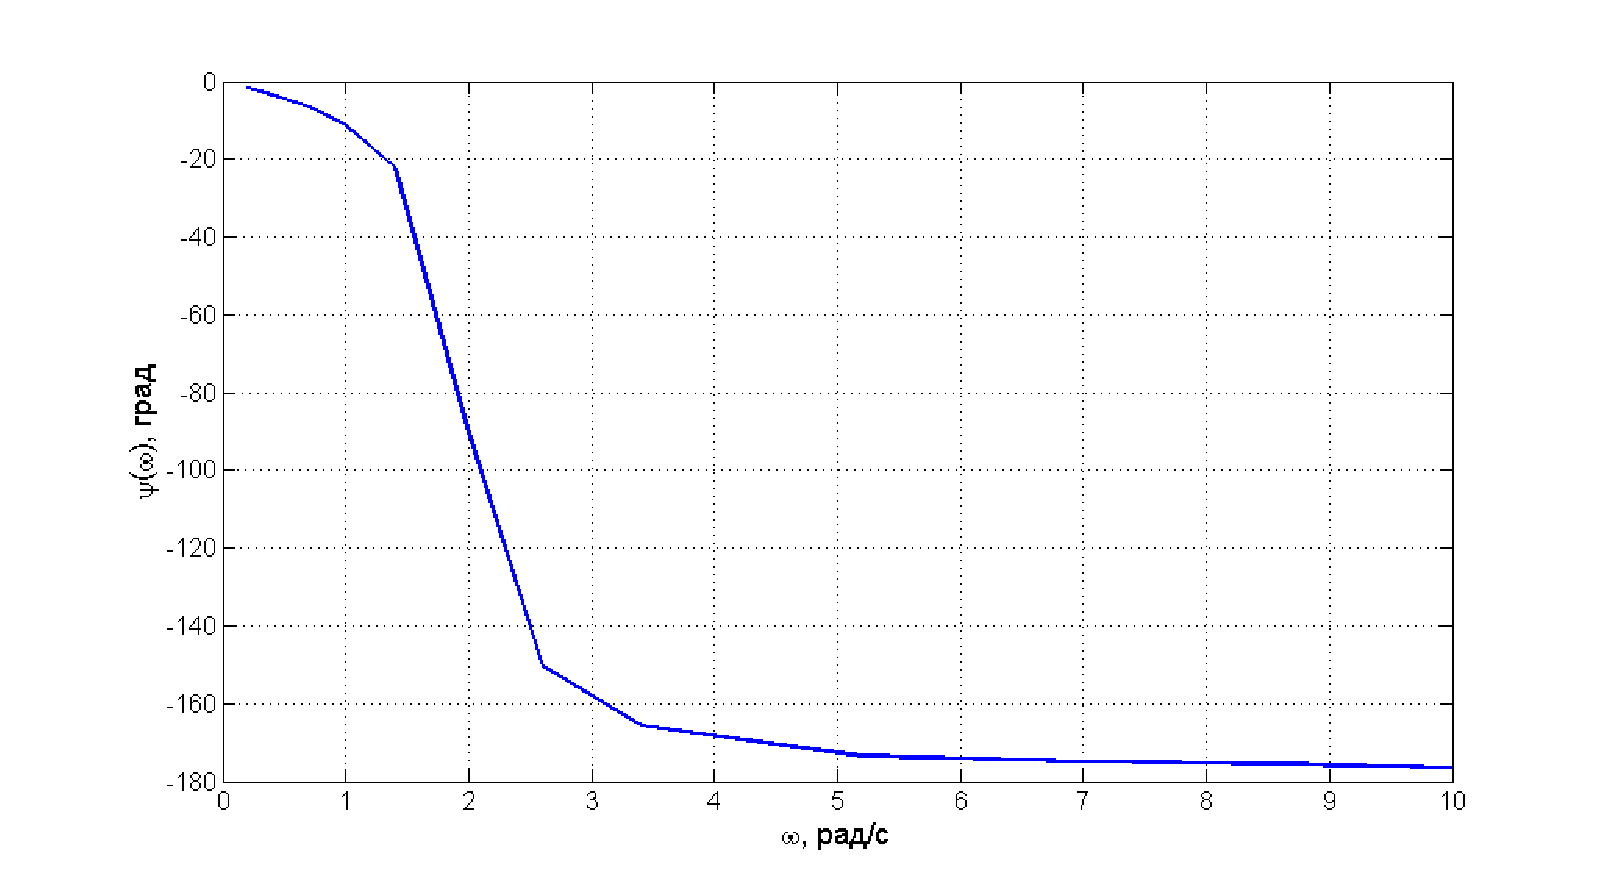
\includegraphics[width=1\linewidth]{FCHH1.eps}
	\caption{ФЧХ}
\end{figure}
\begin{figure}[H]
	\centering
	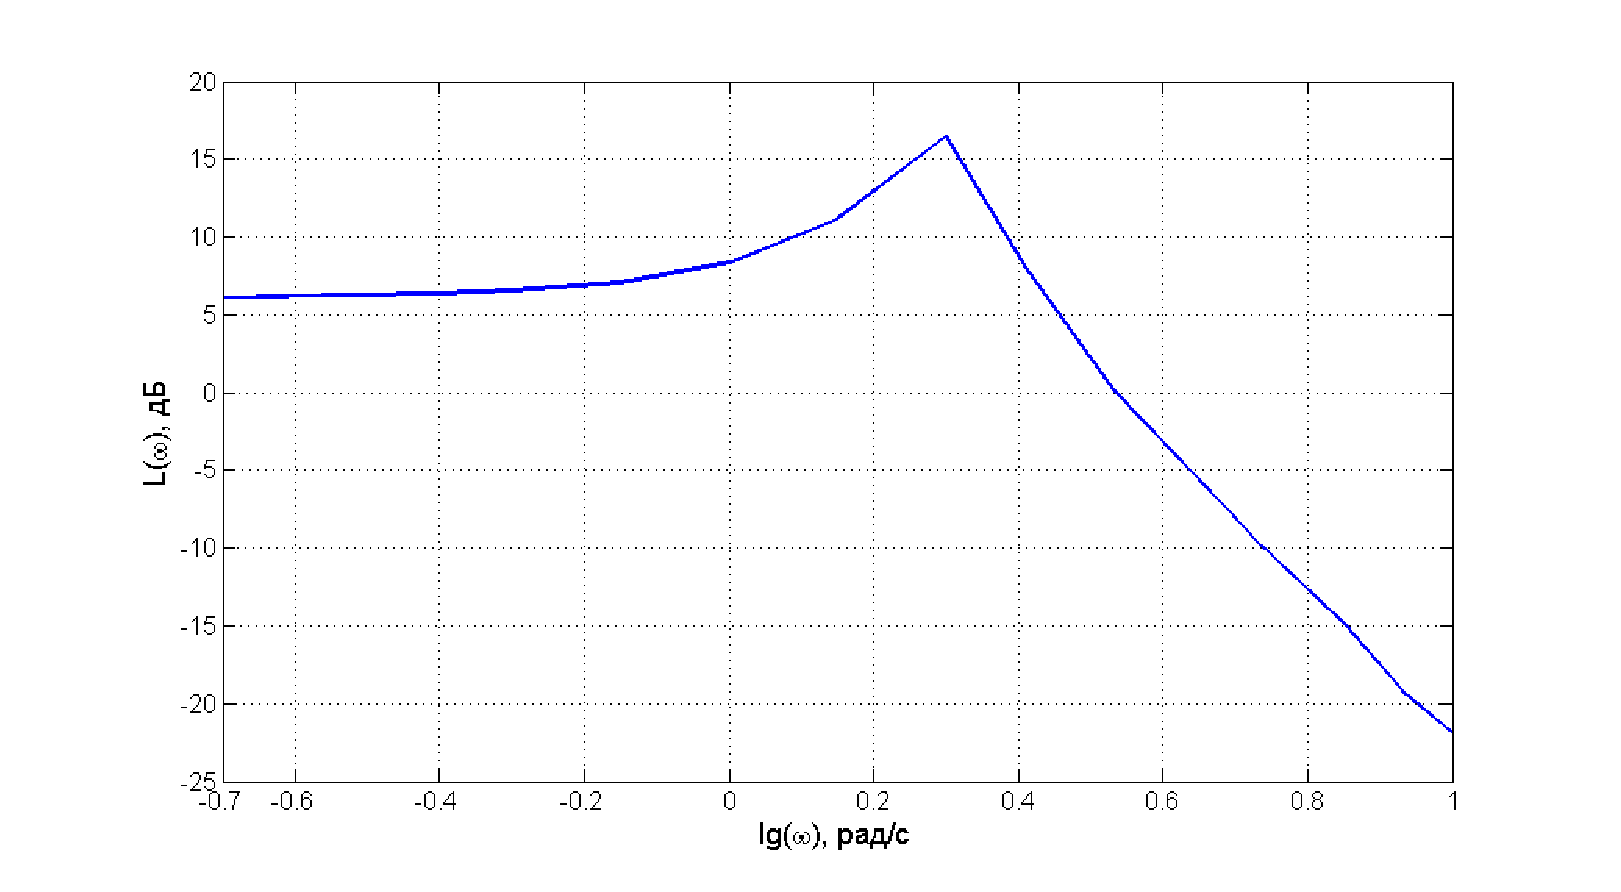
\includegraphics[width=1\linewidth]{LACHH1.eps}
	\caption{ЛАЧХ}
\end{figure}
\begin{figure}[H]
	\centering
	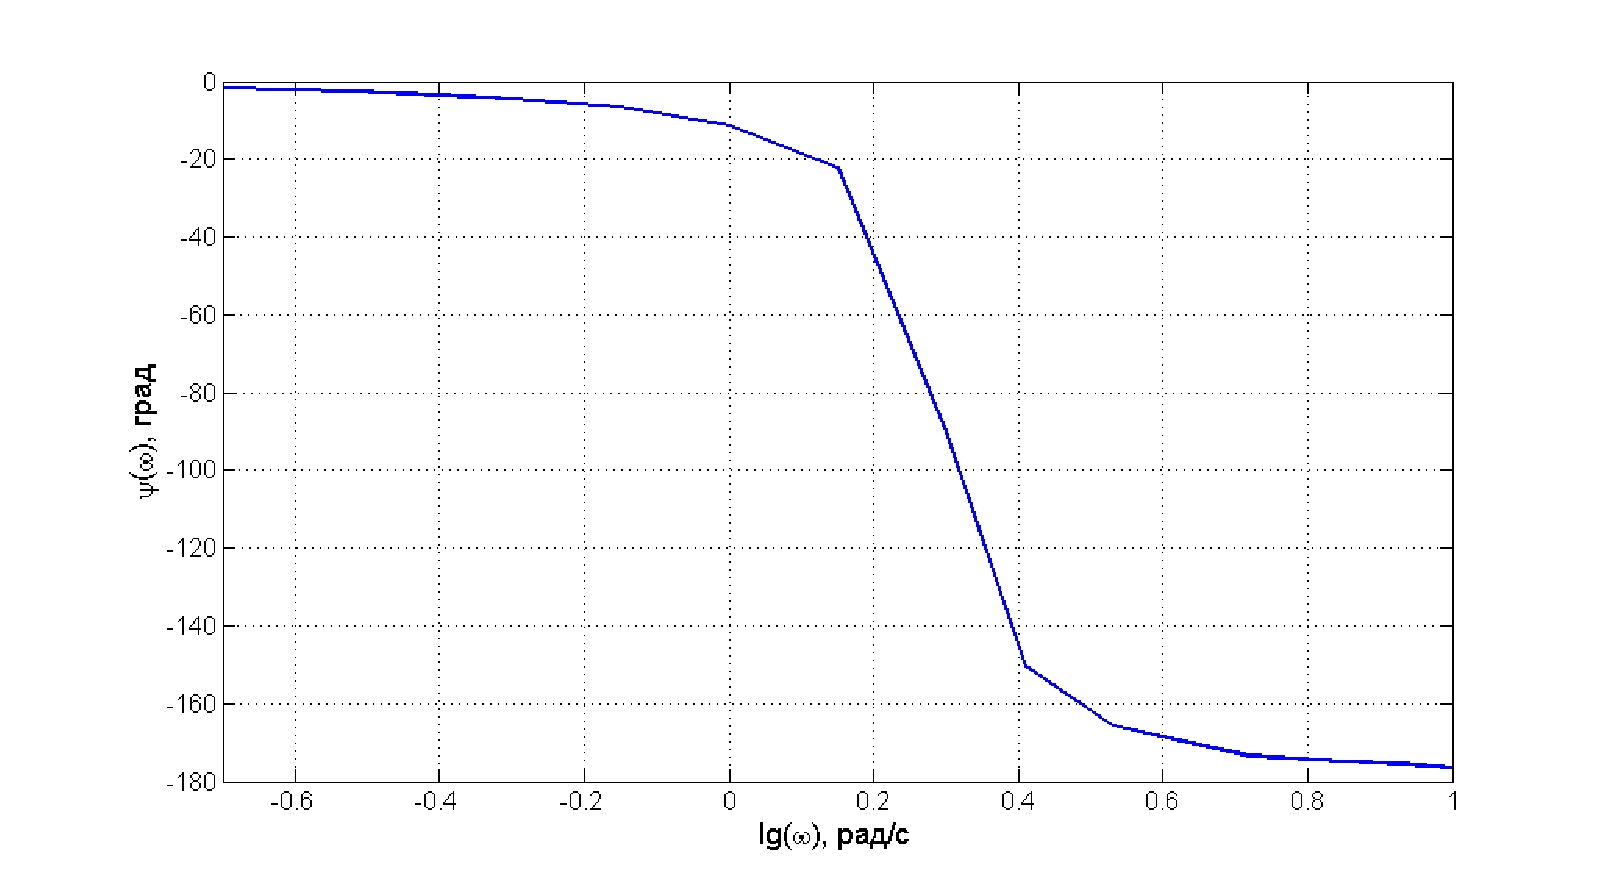
\includegraphics[width=1\linewidth]{LFCHH1.eps}
	\caption{ЛФЧХ}
\end{figure}
\begin{figure}[H]
	\centering
	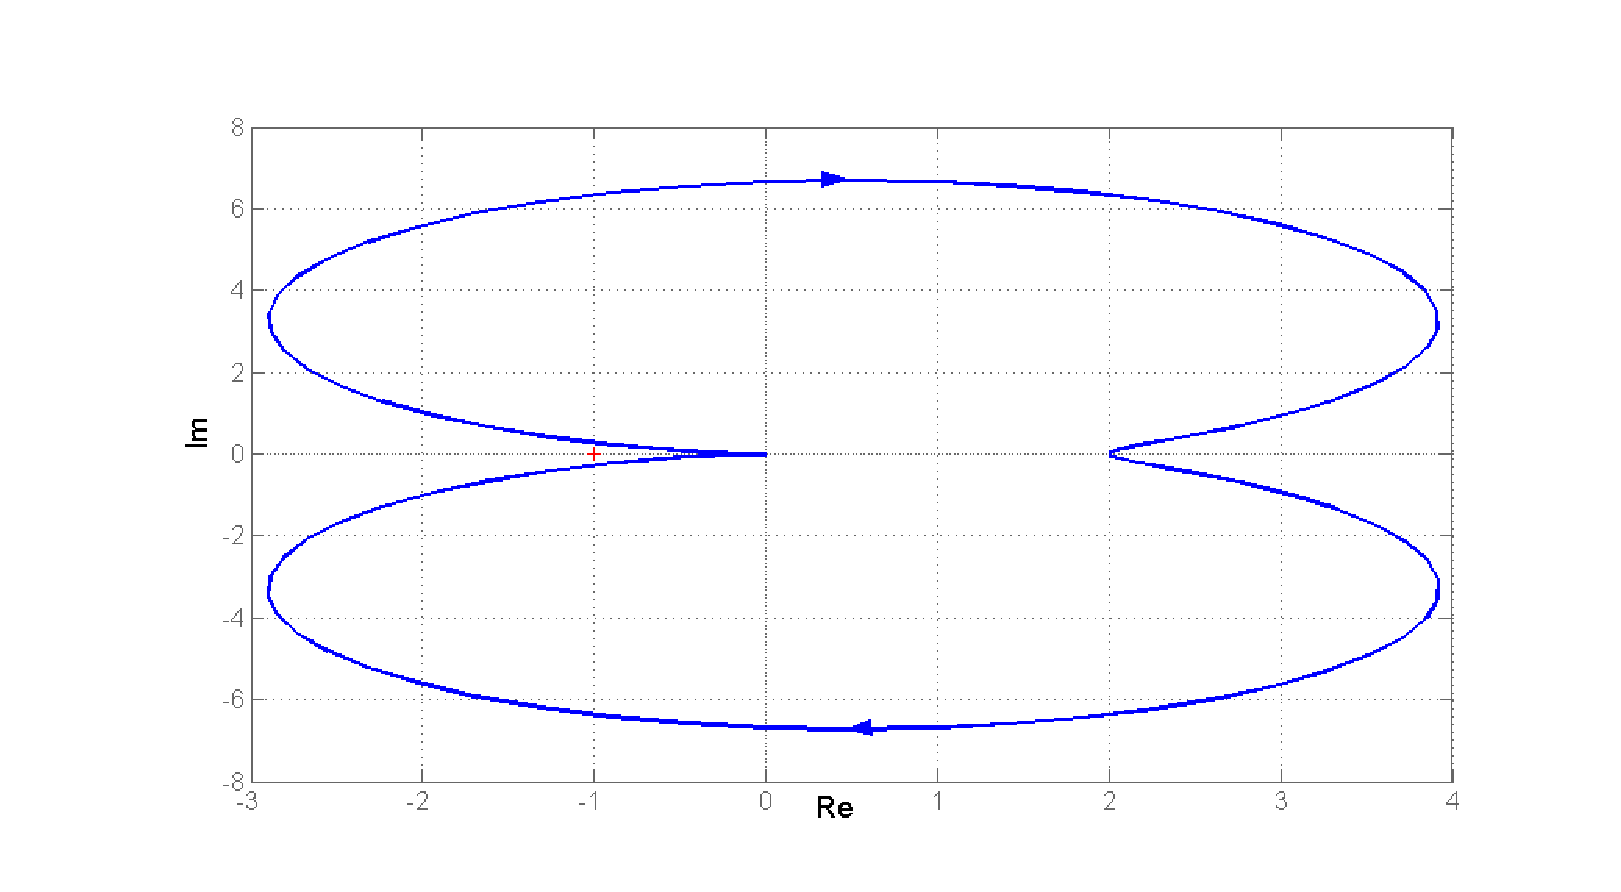
\includegraphics[width=1\linewidth]{AFCHH1.eps}
	\caption{АФЧХ}
\end{figure}
\begin{figure}[H]
	\centering
	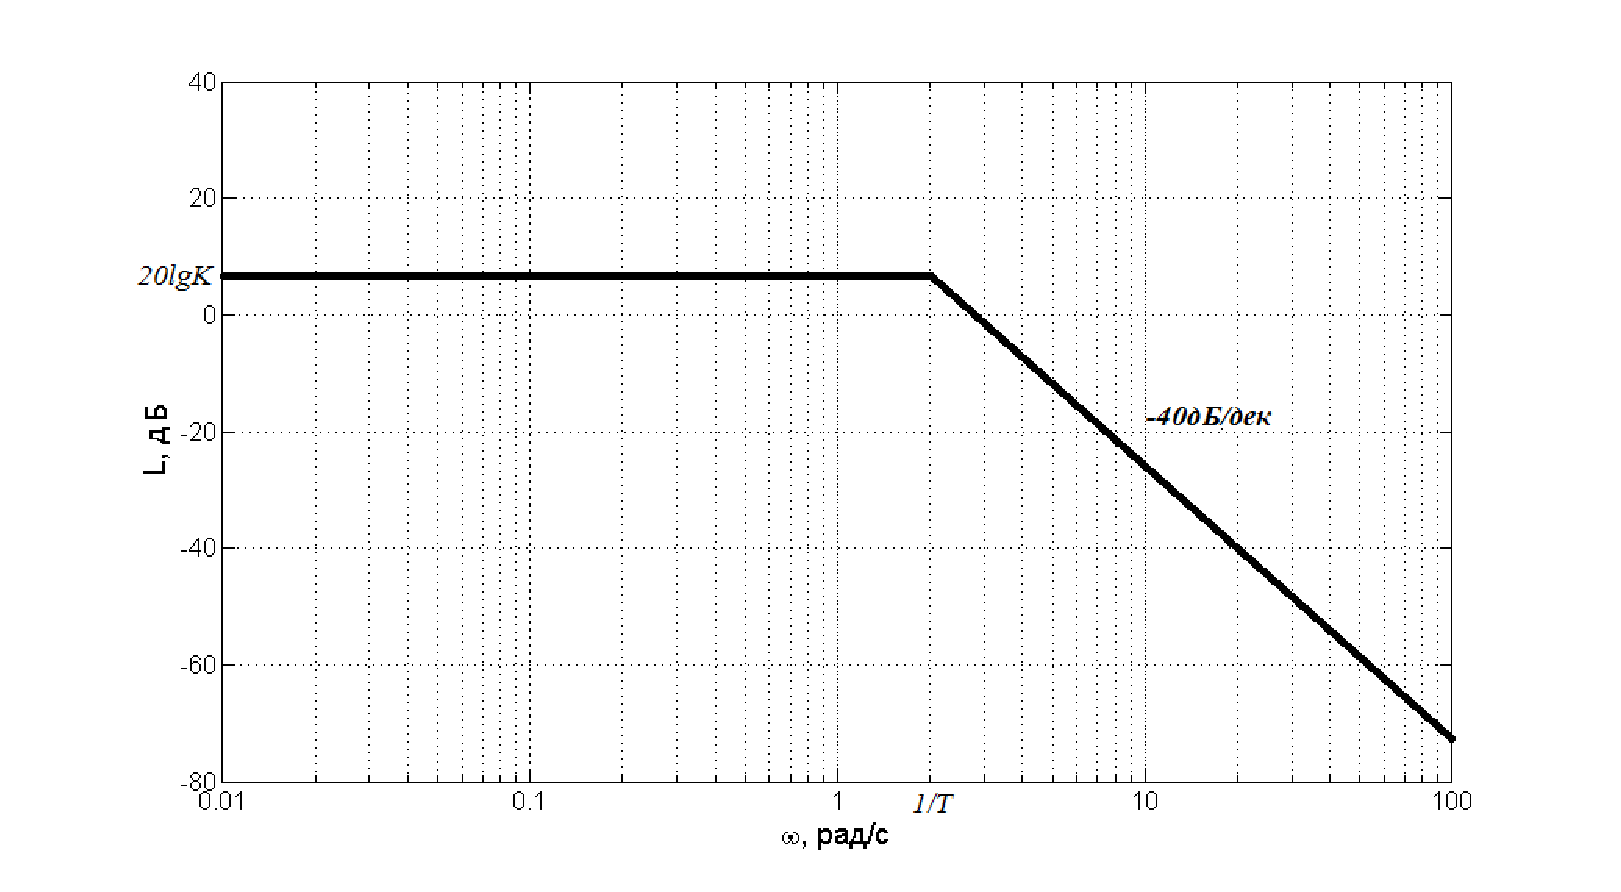
\includegraphics[width=1\linewidth]{L1.eps}
	\caption{Асимптотическая ЛАЧХ}
\end{figure}

\newpage
\begin{center}
\section{Идеальное интегрирующее звено}
\end{center}

В таблице 3 представлены данные при исследовании идеального интегрирующего звена.
\begin{table}[h!]
	\renewcommand{\arraystretch}{1.8} %строки
	\centering
	\begin{threeparttable}
	\caption{Экспериментальные данные для идеального интегрирующего звена}
	\begin{tabular}{|c|c|c|c|c|}
		\hline $\omega$, рад/с & $lg\omega$ & $A(\omega)$ & $L(\omega)=20lgA(\omega)$ & $\psi(\omega)$, град\\
		\hline 0,2 & -0,70 & 10,00 & 20,00 & -90\\
		\hline 0,3 & -0,52 & 6,67 & 16,48 & -90\\
		\hline 0,4 & -0,40 & 5,00 & 13,98 & -90\\
		\hline 0,5 & -0,30 & 4,00 & 12,04 & -90\\
		\hline 0,7 & -0,15 & 2,86 & 9,13 & -90\\
		\hline 1,0 & 0,00 & 2,00 & 6,02 & -90\\
		\hline 1,4 & 0,15 & 1,43 & 3,11 & -90\\
		\hline 2,0 & 0,30 & 1,00 & 0,00 & -90\\
		\hline 2,6 & 0,41 & 0,77 & -2,27 & -90\\
		\hline 3,4 & 0,53 & 0,59 & -4,58 & -90\\
		\hline 5,2 & 0,72 & 0,38 & -8,40 & -90\\
		\hline 7,0 & 0,85 & 0,29 & -10,75 & -90\\
		\hline 8,6 & 0,93 & 0,23 & -12,77 & -90\\
		\hline 10,0 & 1,00 & 0,20 & -13,98 & -90\\
		\hline
	\end{tabular}
	\end{threeparttable}
\end{table}

На рисунках 8-13 представлены частотные характеристики идеального интегрирующего звена.
\begin{figure}[H]
	\centering
	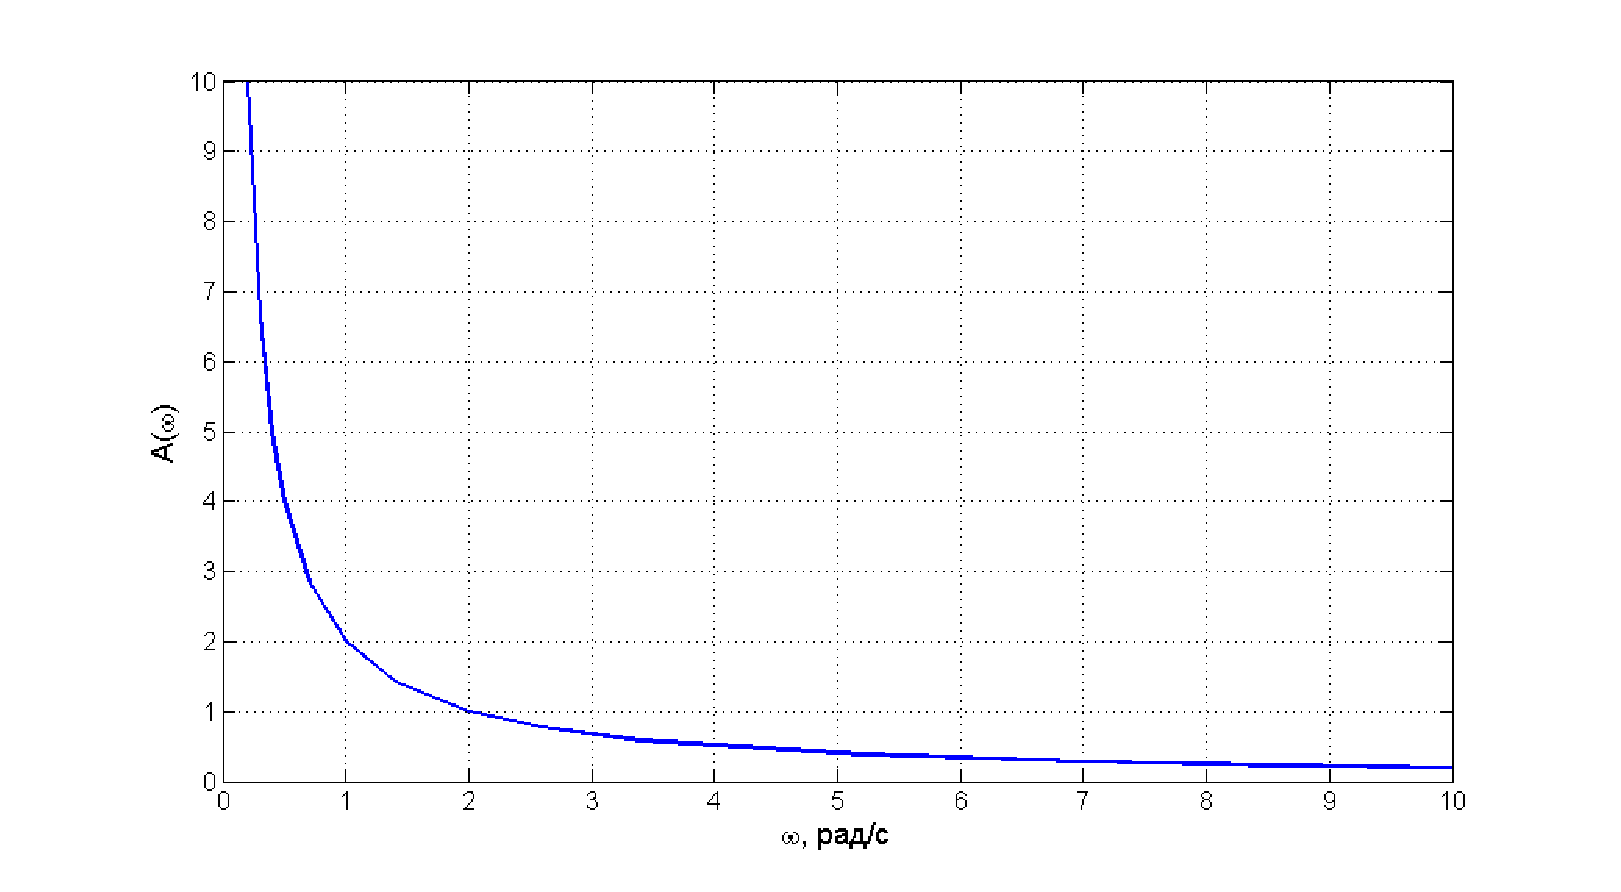
\includegraphics[width=1\linewidth]{ACHH2.eps}
	\caption{АЧХ}
\end{figure}
\begin{figure}[H]
	\centering
	\includegraphics[width=1\linewidth]{FCHH2.eps}
	\caption{ФЧХ}
\end{figure}
\begin{figure}[H]
	\centering
	\includegraphics[width=1\linewidth]{LACHH2.eps}
	\caption{ЛАЧХ}
\end{figure}
\begin{figure}[H]
	\centering
	\includegraphics[width=1\linewidth]{LFCHH2.eps}
	\caption{ЛФЧХ}
\end{figure}
\begin{figure}[H]
	\centering
	\includegraphics[width=1\linewidth]{AFCHH2.eps}
	\caption{АФЧХ}
\end{figure}
\begin{figure}[H]
	\centering
	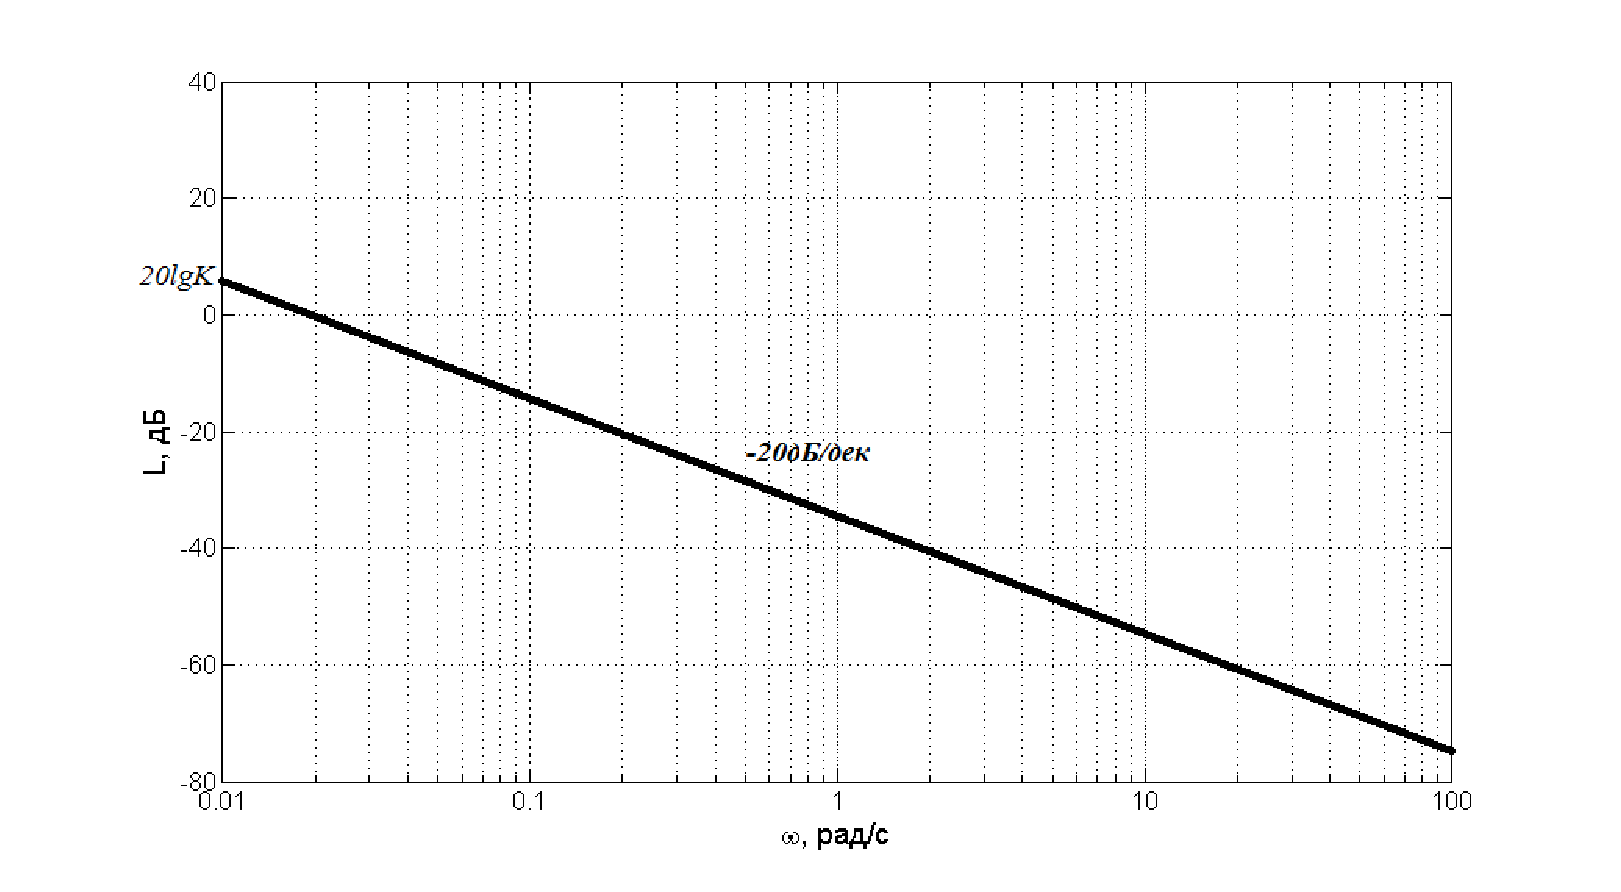
\includegraphics[width=1\linewidth]{L2.eps}
	\caption{Асимптотическая ЛАЧХ}
\end{figure}

\newpage
\begin{center}
\section{Изодромное звено}
\end{center}

В таблице 4 представлены данные при исследовании изодромного звена.
\begin{table}[h!]
	\renewcommand{\arraystretch}{1.8} %строки
	\centering
	\begin{threeparttable}
	\caption{Экспериментальные данные для изодромного звена}
	\begin{tabular}{|c|c|c|c|c|}
		\hline $\omega$, рад/с & $lg\omega$ & $A(\omega)$ & $L(\omega)=20lgA(\omega)$ & $\psi(\omega)$, град\\
		\hline 0,2 & -0,70 & 10,05 & 20,04 & -84,22\\
		\hline 0,3 & -0,52 & 6,74 & 16,57 & -81,36\\
		\hline 0,4 & -0,40 & 5,10 & 14,15 & -78,50\\
		\hline 0,5 & -0,30 & 4,12 & 12,30 & -76,20\\
		\hline 0,7 & -0,15 & 3,03 & 9,63 & -70,47\\
		\hline 1,0 & 0,00 & 2,24 & 7,00 & -63,60\\
		\hline 1,4 & 0,15 & 1,74 & 4,81 & -55,00\\
		\hline 2,0 & 0,30 & 1,41 & 2,98 & -45,00\\
		\hline 2,6 & 0,41 & 1,26 & 2,01 & -37,82\\
		\hline 3,4 & 0,53 & 1,16 & 1,29 & -30,37\\
		\hline 5,2 & 0,72 & 1,07 & 0,59 & -20,63\\
		\hline 7,0 & 0,85 & 1,04 & 0,34 & -16,04\\
		\hline 8,6 & 0,93 & 1,03 & 0,26 & -13,18\\
		\hline 10,0 & 1,00 & 1,02 & 0,17 & -11,46\\
		\hline
	\end{tabular}
	\end{threeparttable}
\end{table}

На рисунках 14-19 представлены частотные характеристики изодромного звена.
\begin{figure}[H]
	\centering
	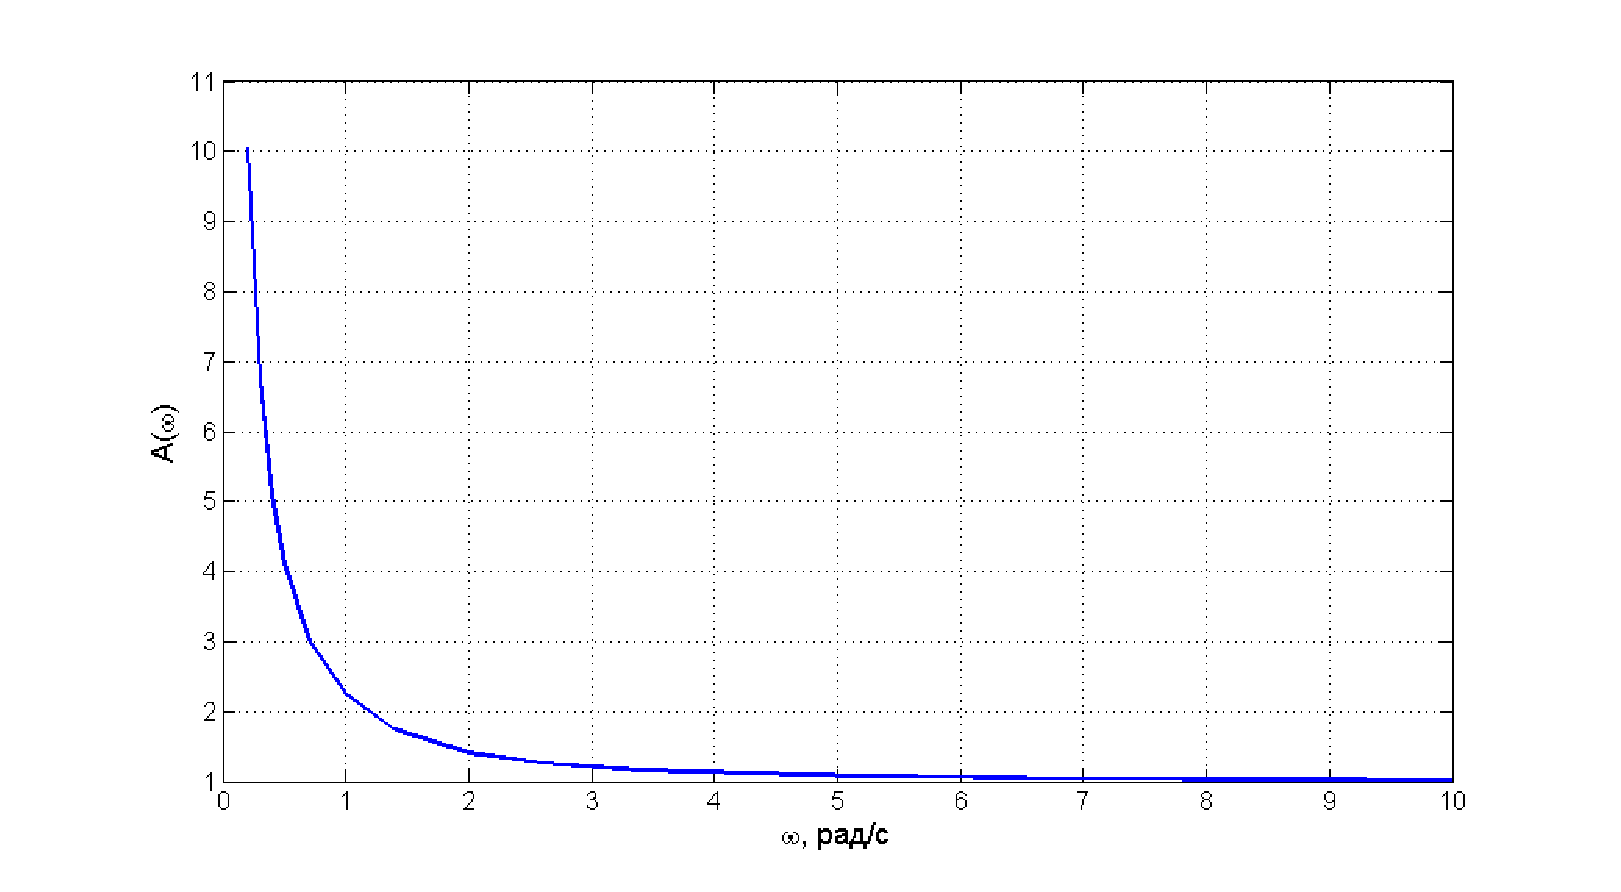
\includegraphics[width=1\linewidth]{ACHH3.eps}
	\caption{АЧХ}
\end{figure}
\begin{figure}[H]
	\centering
	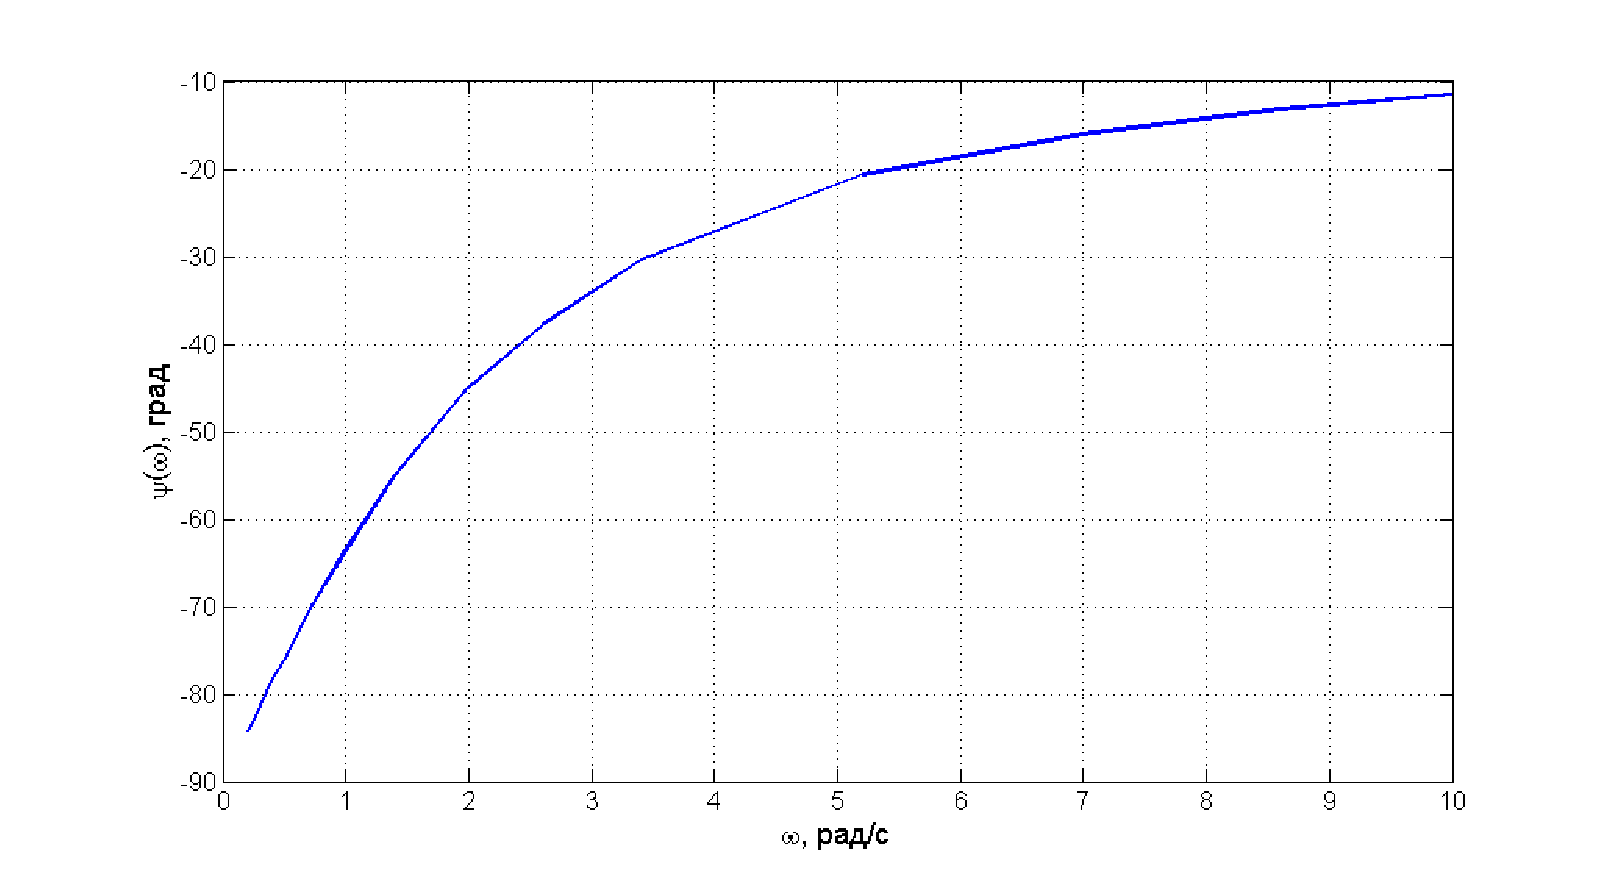
\includegraphics[width=1\linewidth]{FCHH3.eps}
	\caption{ФЧХ}
\end{figure}
\begin{figure}[H]
	\centering
	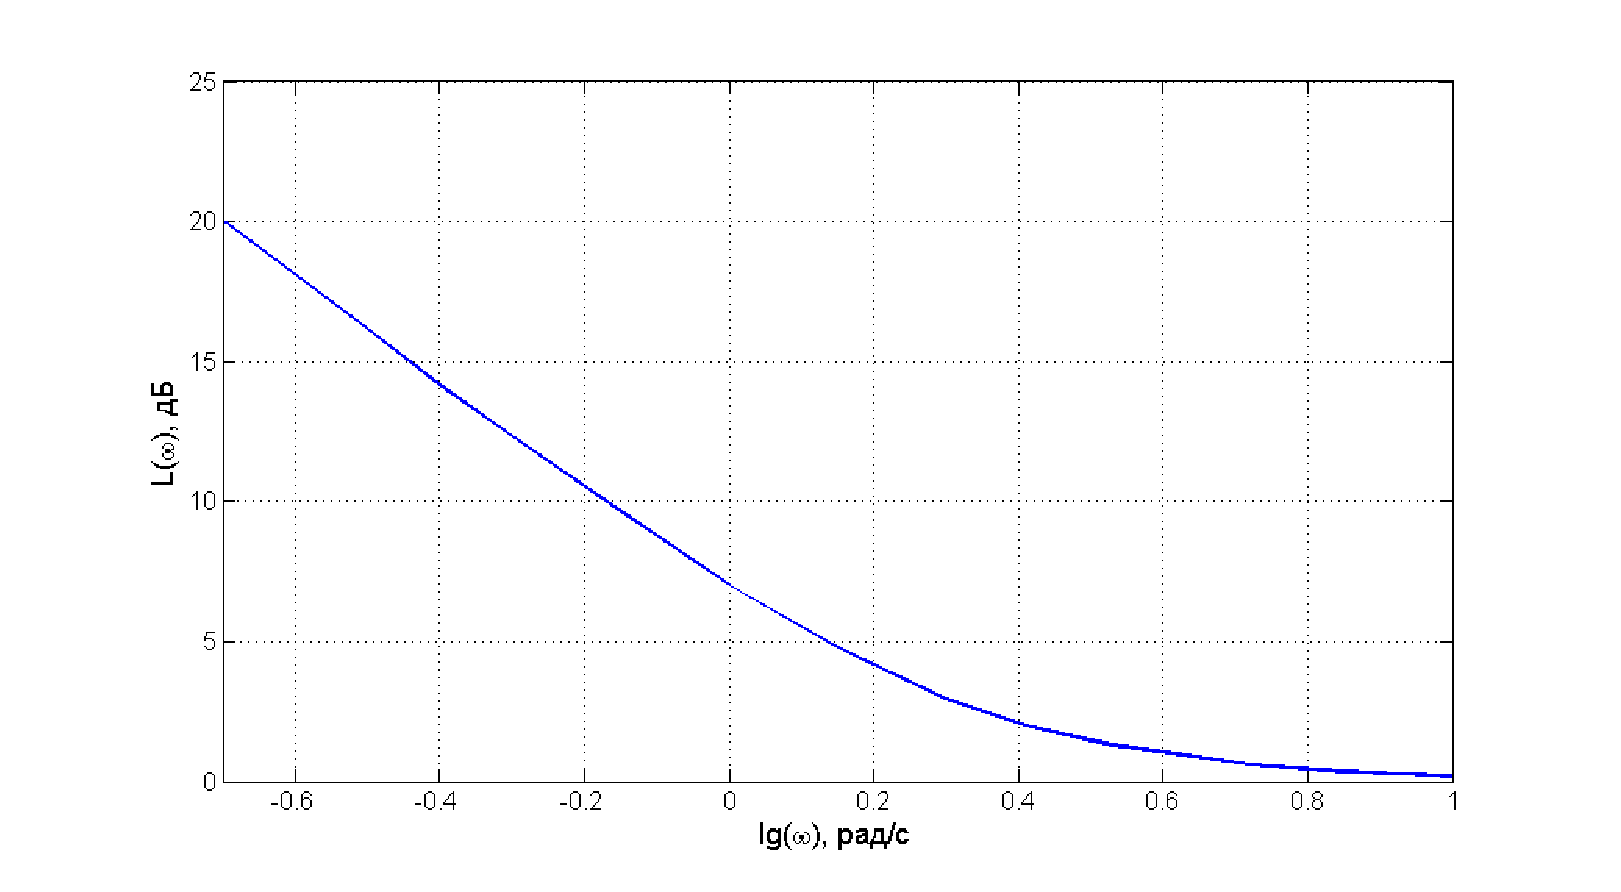
\includegraphics[width=1\linewidth]{LACHH3.eps}
	\caption{ЛАЧХ}
\end{figure}
\begin{figure}[H]
	\centering
	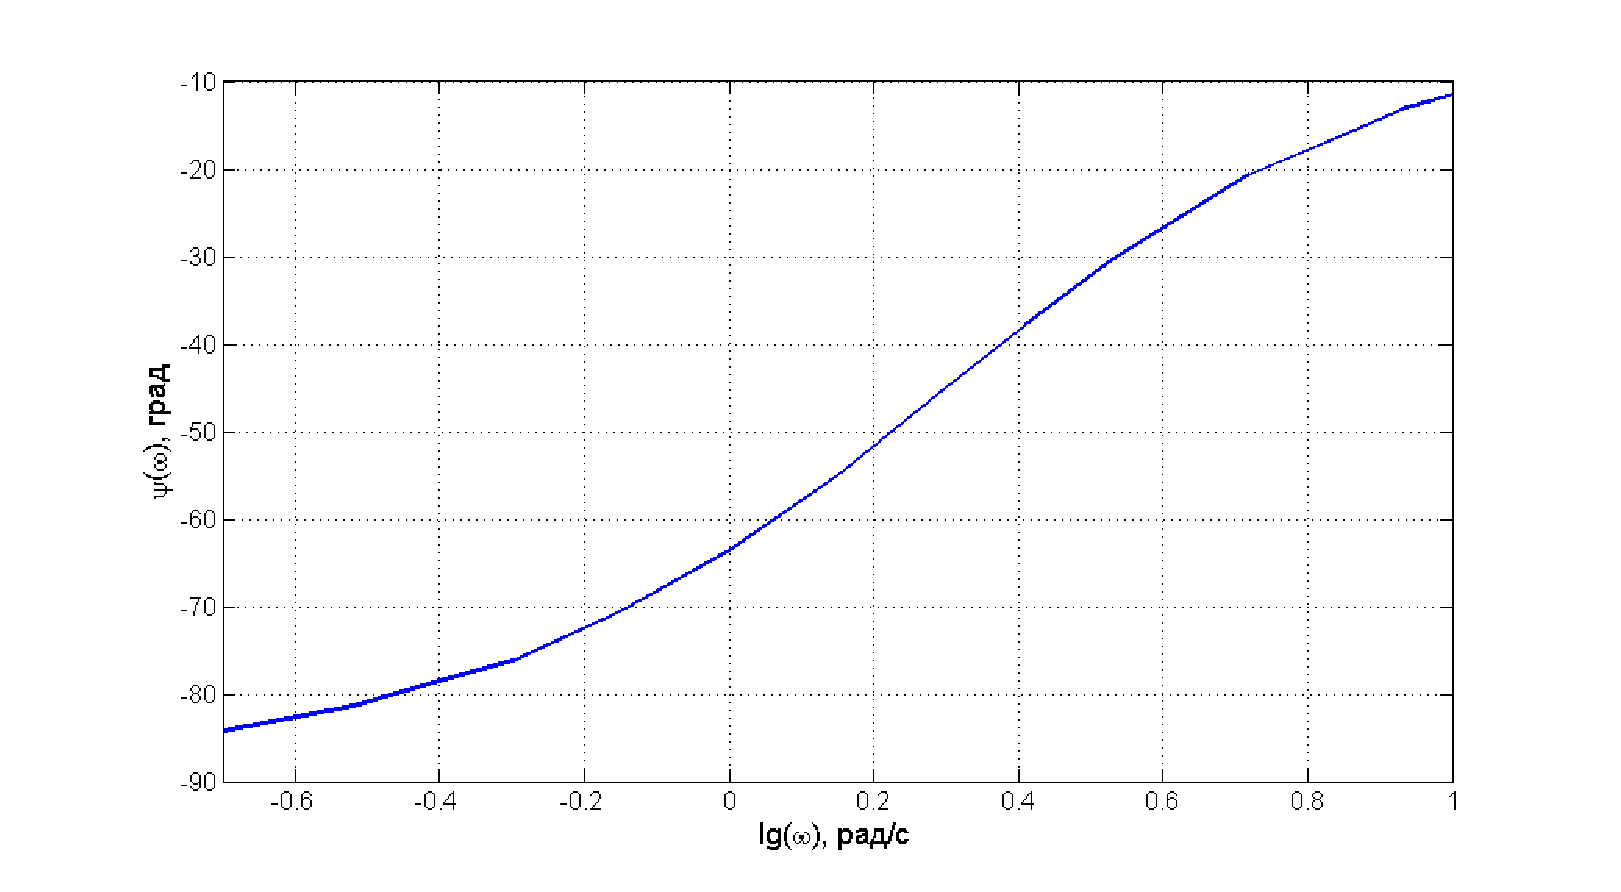
\includegraphics[width=1\linewidth]{LFCHH3.eps}
	\caption{ЛФЧХ}
\end{figure}
\begin{figure}[H]
	\centering
	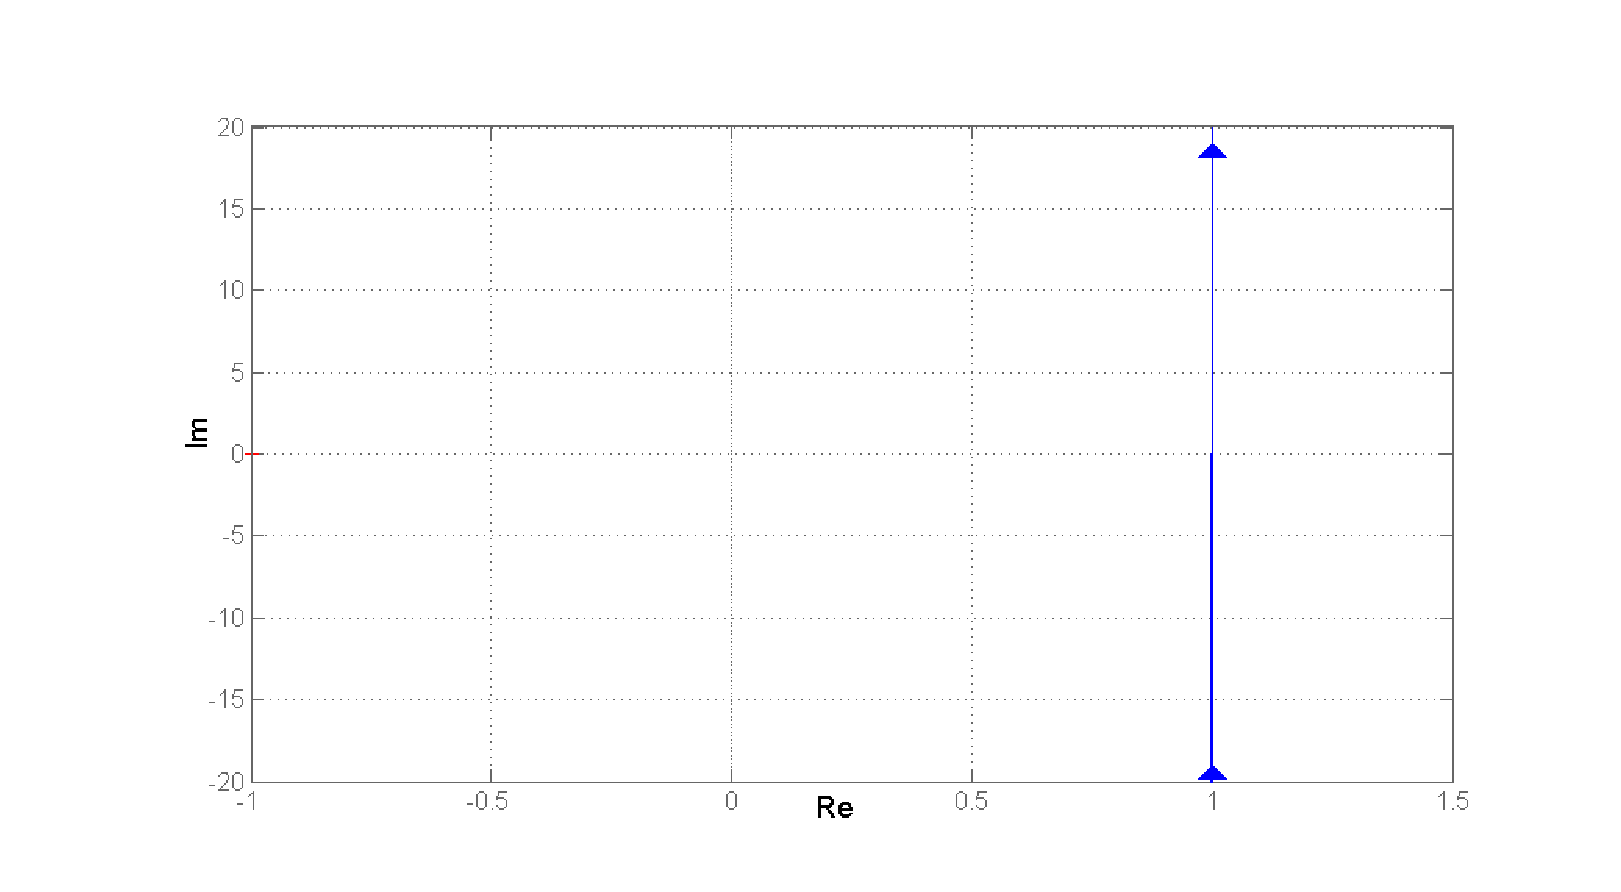
\includegraphics[width=1\linewidth]{AFCHH3.eps}
	\caption{АФЧХ}
\end{figure}
\begin{figure}[H]
	\centering
	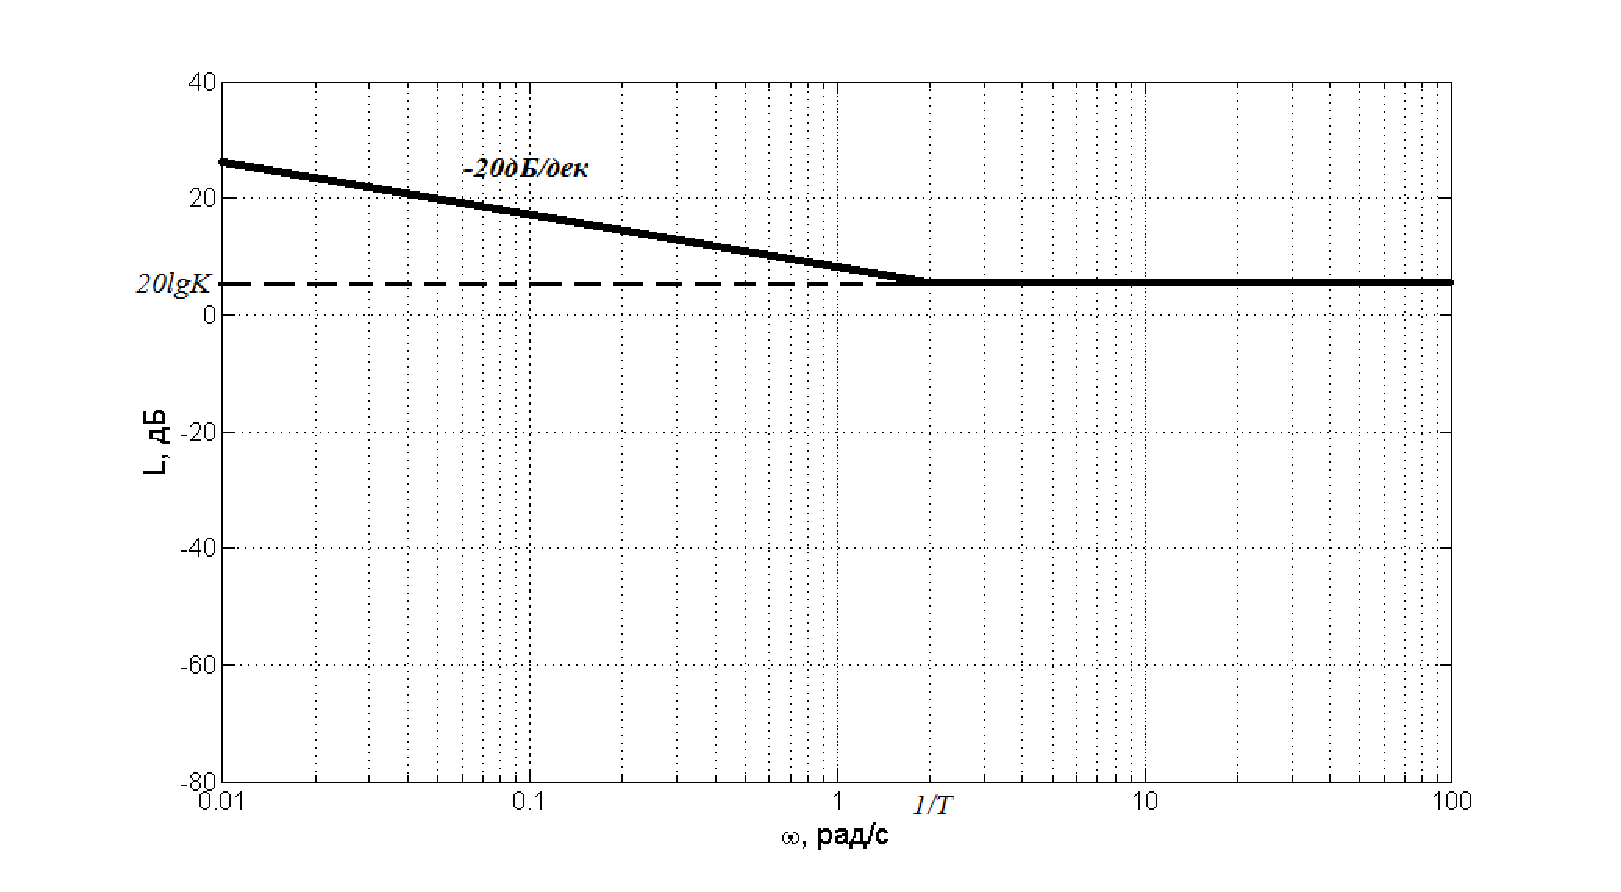
\includegraphics[width=1\linewidth]{L3.eps}
	\caption{Асимптотическая ЛАЧХ}
\end{figure}

\newpage
\section*{Вывод}
В ходе лабораторной работы были изучены частотные и логарифмические частотные характеристики типовых динамических звеньев: колебательного, идеального интегрирующего и изодромного.
Основываясь на экспериментальных данных можно говорить о том, что фазовый сдвиг для колебательного звена изменяется в пределах от $0^{\circ}$ до $-180^{\circ}$, для изодромного --- от $-90^{\circ}$ до $0^{\circ}$, а для идеального интегрирующего звена фазовый сдвиг равен $-90^{\circ}$.\par
Сравнивая графики ЛАЧХ и асимптотической ЛАЧХ, можно заметить, что асимптотические ЛАЧХ сходятся к реальным ЛАЧХ, и с их помощью удобно проводить синтез систем управления.\par
Также можно сделать вывод о том, что асимптотическая ЛАЧХ меняет свой наклон при частоте среза $\omega_c = 1/T$ и для её построения не требуется выполнения дополнительных вычислений, достаточно лишь знать вид передаточной функции.Также по асимптотический ЛАЧХ можно восстановить передаточную функцию.  
\end{document}